% This is samplepaper.tex, a sample chapter demonstrating the
% LLNCS macro package for Springer Computer Science proceedings;
% Version 2.20 of 2017/10/04
%
\documentclass[runningheads]{llncs}

\usepackage{graphicx}

\usepackage{cite}
\usepackage{amsmath}
\usepackage{booktabs}
\usepackage{algorithm}
\usepackage[noend]{algpseudocode}
\usepackage{booktabs}
\usepackage{footnote}
\usepackage{xcolor}
\makesavenoteenv{tabular}
\makesavenoteenv{table}
\usepackage{multirow}
\usepackage{hhline}
\usepackage{array}
\usepackage{amsmath}
\usepackage{amssymb}
% \scalebox{algorithm}
\usepackage{marvosym}

\DeclareMathOperator*{\argmax}{arg\,max}

\begin{document}
%
\title{Accelerating Substructure Similarity Search for Formula Retrieval}
\titlerunning{Accelerating Substructure Similarity Search}

\author{Wei Zhong\inst{1}\textsuperscript{,\Letter}, Shaurya Rohatgi\inst{2}, Jian Wu\inst{3}, C. Lee Giles\inst{2} \and Richard Zanibbi\inst{1}\textsuperscript{,\Letter}}
\institute{
Rochester Institute of Technology \\
\email{\{wxz8033,rxzvcs\}@rit.edu}
\and Pennsylvania State University 
\and Old Dominion University
}

\authorrunning{Wei Zhong et al.}

\maketitle

\begin{abstract}
Existing formula retrieval systems that use substructure matching are effective, but suffer from slow retrieval times caused by the complexity of structure matching.  We present a specialized inverted index structure and rank-safe dynamic pruning algorithm for faster substructure retrieval. Formulas are indexed from their Operator Tree (OPT) presentations. Our model is evaluated on the NTCIR-12 Wikipedia Formula Browsing Task dataset and a newly created larger formula corpus crawled from Math StackExchange.  Our results show that
our approach preserves the effectiveness of structure matching, while also allowing queries to be executed in real-time.

\keywords{Math information retrieval, Query processing optimization, Dynamic pruning}
\end{abstract}

\section{Introduction}
In information retrieval, a great deal of research has gone into creating efficient search engines for large corpora.
However, a few of them have addressed substructure search in structural content, e.g., in Mathematical Information Retrieval (MIR)~\cite{survey2012} where efficient substructure similarity search is needed to to identify shared subexpressions effectively.
For example, in math expression search problem, to discern that $a+b$ and $b + a$ are equivalent (by commutativity), but that $ab+cd$ and $a+bcd$ are different, simply applying tokenization and counting common token frequencies are not sufficient. Instead, a hierarchical representation of mathematical operations is needed, shared substructures also need to be identified.

%%%%%%%%%%%%%%%%%%%%%%%%%%%%%%%%%%%%%%%%%%%%%%%%%%%%%%%%%%%%%%
\begin{figure}[!t]

\begin{center}
\begin{minipage}[b]{1.5in}
\begin{center}
\includegraphics[width=1.2in]{fig/tree3.eps}\\
$bc + xy + a + z$
\end{center}
\end{minipage}
\hspace*{.0in}
\begin{minipage}[b]{1.5in}
\begin{center}
\raisebox{.0in}{\includegraphics[width=0.9in]{fig/tree4.eps}}\\
$(a + bc) + xy$
\end{center}
\end{minipage}
\end{center}

\caption{Operator trees (OPTs) for two similar formulas. OPTs represent the application of operations (at internal nodes in circles) to operands (at the leaves in squares). Two common substructures are highlighted in green and purple.}
\label{intro}
\end{figure}
%%%%%%%%%%%%%%%%%%%%%%%%%%%%%%%%%%%%%%%%%%%%%%%%%%%%%%%%%%%%%%

In the most recent math similarity search competition\footnote{The NTCIR-12 Wikipedia Formula Browsing Task.}, effective systems all take a tree-based approach by extracting query terms from tree representations.
For example, an Operator Tree (OPT) is used in Figure~\ref{intro} to represent math formulas where operands are represented by leaves and operators are lifted to the internal nodes.
This facilitates searching the common subtrees shared by two math expressions, specifically, we can index paths from their tree representations and find their shared structure by matching their common paths grouped by root-end nodes. 
However, indexing all prefixes of leaf-root paths would result in considerable query terms in any realistic math search task. In order to carry structure information, it is common to see long queries with over tens or even hundreds of ``terms" which is unusual for text search. This makes query processing costly because many posting lists are merged for retrieval.

In text similarity search, query processing can be accelerated through dynamic pruning~\cite{tonellotto2018efficient}, which typically estimates score upperbounds to prune documents unlikely to be in the top K results.

However, effective substructure search requires additional matching or alignment among query terms, and this makes it hard to get a good score estimation thus it prevents us applying traditional dynamically pruning effectively.
In fact, reportedly few state-of-the-art MIR systems have achieved practical query run times even when given a large amount of computing resources~\cite{ntcir12, mcat_16}.
In this paper we try to address this problem by introducing a specialized inverted index and we propose a dynamic pruning method based on this specialized inverted index to boost efficiency.

%%%%%%%%%%%%%%%%%%%%%%%%%%%%%%%%%%%%%%%%%%%%%%%%%%%%%%%%%%%%%%
% \begin{figure}[!t]
% \begin{center}
% 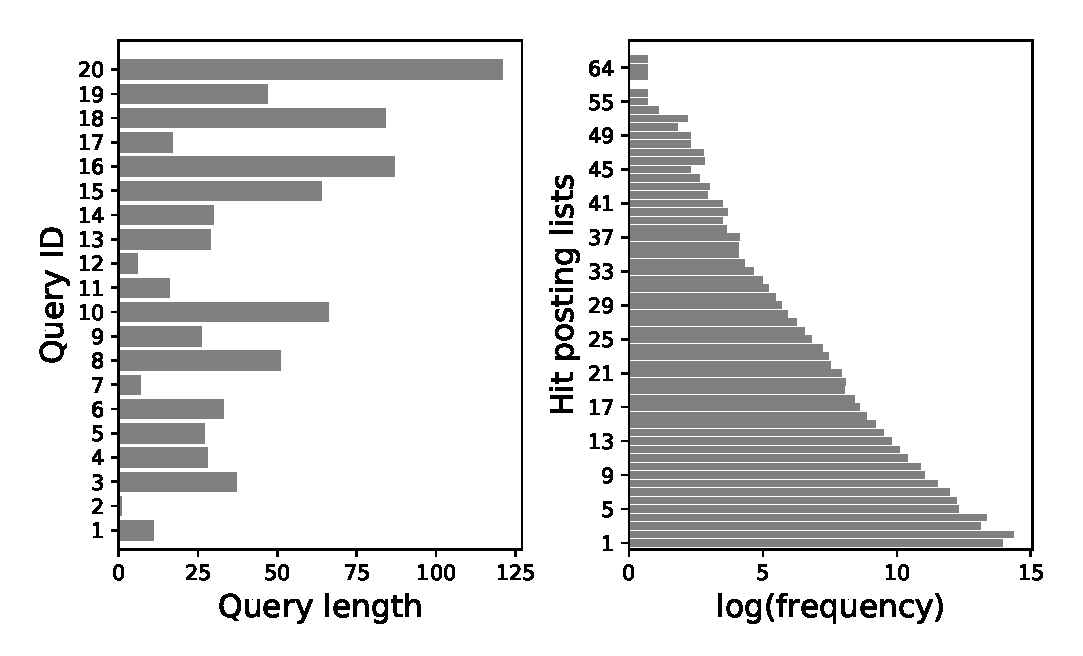
\includegraphics[width=2.2in]{fig/hot-hit.eps}
% \caption{Non-wildcards query statistics produced by a tree-based system~\cite{a0_2019} in the NTCIR-12 Wikipedia Formula Browsing Task.
% %At left are the number of leaft-root sub-paths (query terms) produced for the 20 queries, while at right the posting list hit frequencies are shown.
% }
% \label{stats}
% \end{center}
% \end{figure}
%%%%%%%%%%%%%%%%%%%%%%%%%%%%%%%%%%%%%%%%%%%%%%%%%%%%%%%%%%%%%%

\section{Related Work}
\label{relatedworks}

Recently there has been an increasing amount of research on similarity search for math formulas, with most focusing on search effectiveness~\cite{a0_2019,tangent-combine2017,mcat_16,peking2016}.
There are many emerging issues regarding effectiveness, including handling mathematical semantics, and identifying interchangeable symbols and common subexpressions. However, the efficiency of math formula search systems is often not addressed.

%
A number of MIR systems apply text search models to math retrieval, extracting sequential features from formulas and use TF-IDF variants scoring~\cite{nist_03, mias_11, peking2014}. These approaches incorporate a bag-of-words model, and use frequency to measure formula similarity. Inevitably, they need to index different combinations of sequences or substrings to handle operator commutativity and associativity.
This index augmentation results in a non-linearly increasing index size in the number of indexed ``words''~\cite{peking2014} and thus hurts efficiency for large corpora.
%
On the other hand, recent results~\cite{ntcir12, a0_2019, tangent_2019} reveal that effective systems for formula retrieval use tree-based approaches distinct from text-based methods.
%
However, tree-based systems usually need to calculate costly graph matching or edit distance metrics~\cite{tangent-multistage2016, edit_dist2013}, which generally have non-linear time complexity.
Recently, a path-based approach~\cite{a0_2019} was developed to search substructures in formula OPTs approximately by assuming that identical formulas have the same leaf-root path set.
Although it obtains the best effectiveness for the NTCIR-12 dataset, due to a typically large number of query paths in formula subtrees, the query run time performance is still not ideal (the maximum run times can take a couple of seconds).

Dynamic pruning has been recognized as an effective way to reduce query processing times~\cite{jonassen_simon_2011, antonio2019, macdonald2011upper, tonellotto2018efficient}.
%
Dynamic pruning speeds up query processing by skipping scoring calculations or avoiding unnecessary reads for documents which are unlikely to be ranked into the top K results.
%
Pruning methods can be based on different query processing schemes:
Document-at-a-time (DAAT) requires all relevant posting lists be merged simultaneously. Term-at-a-time (TAAT) or score-at-a-time (SAAT) processes one posting list at a time for each term, requiring additional memory to store partial scores, and posting lists in this case are usually sorted by document importance (e.g, impact score~\cite{anh2006SAAT}), with promising documents placed at  the front of inverted lists.
%
Pruning strategies are \textit{rank-safe} (or \textit{safe up to rank K})~\cite{turtle_flood_1995} if they guarantee that the top K documents are ranked in the same order before and after pruning. 
%
The most well-known rank-safe pruning strategies for DAAT are MaxScore~\cite{turtle_flood_1995, strohman_turtle_2005, jonassen_simon_2011} and WAND variants~\cite{broder2003WAND, ding2011BMW}.
%\footnote{MaxScore also has TAAT version~\cite{turtle_flood_1995}.} 
%
Shan et al.~\cite{Shandongdong2012} show that MaxScore variants (e.g. BMM, LBMM) outperform other dynamic pruning strategies for long queries, and recently Mallia et al.~\cite{antonio2019} report a similar finding over a range of popular index encodings.


%%%%%%%%%%%%%%%%%%%%%%%%%%%%%%%%%%%%%%%%%%%%%%%%%%%%%%%%%%%
\section{Preliminaries}
\noindent\textbf{Baseline Model}\; This work is based on our previous work~\cite{a0_2019} which extracts prefixes from query OPT leaf-root paths as query or index terms, the OPT is parsed from a formula/expression in \LaTeX{}. For indexed paths, they are mapped to corresponding posting lists in an inverted index where the IDs of expressions containing the path are appended.
At query time, the posting lists corresponding to query formula paths are merged and approximate matching is performed on candidates one expression at a time.

Because math symbols are interchangeable, paths are tokenized for better recall (operand symbols such as $a, b, c$ are tokenized into VAR).
Given Figure~\ref{intro} for example, if document expression ``bc + xy + a + z'' is indexed, its expression ID (or ExpID) will be appended to the posting lists associated with tokenized paths from its OPT representation.
And the two common structures highlighted in green and purple can be found by matching these tokenized paths, i.e.,  VAR/TIMES, VAR/ADD and VAR/TIMES/ADD (uppercase words denote tokens, VAR is the token for variables) and group them by shared subtree root nodes (i.e., ADD and TIMES on the right side) as proposed in \cite{a0_2019}.
%
In our context, two paths can match if and only if they have the same tokenized paths,
hence ``a/+'' and ``z/+'' can be matched.

As a result, in addition to expression IDs, the posting list entry stores the root-end node IDs of indexed paths to reconstruct structure at merge time.
At query time, the model use the size of matched common subtrees, assuming that subtrees are structurally identical only if their leaf-root paths match.

The model then chooses a subset of widest matched subtree(s) (e.g., $a+bc$ is the maximum one since it has 3 common leaves and is ``wider'' than the other choices) and score similarity based on their properties (e.g. by the total number of matched nodes).

The original model proposes to match as many as 3 widest common subtrees and measure similarity by summing the number of matched leaves and operators from different common subtrees $\hat{T}_q^i, \hat{T}_d^i$ of a common forest $\pi$ (assigning them different score weights $\alpha$ and $\beta$):
\begin{align}
\label{eq:1}
\sum_{(\hat{T}_q^i, \hat{T}_d^i) \in \pi} \beta_i \left( \alpha \left|\operatorname{internals}(\hat{T}_d^i)\right| + (1 - \alpha) \left|\operatorname{leaves}(\hat{T}_d^i)\right| \right) 
\end{align}

%
According to previous experiments in \cite{a0_2019}, interestingly, the multiple subtree matching does boost effectiveness, but matching only single widest common subtree would still produce results that outperform other systems in highly relevance metrics.
%
Consider only scoring based on the widest common subtree and counting its operands, the scoring can be much more simplified, and the resulting score between query and document OPTs $T_q, T_d$ is the widest matched tree width $w^*_{Q, D}$, formally
\begin{align}
\label{eq:2}
w^*_{Q, D} = \max(|\operatorname{leaves}(\hat{T}_d)|), \quad \hat{T}_q, \hat{T}_d \in \text{CFS}(T_q, T_d)
\end{align}
where
$\text{CFS}(T_q, T_d)$ are all the \textit{common formula subtrees} between $T_q$ and $T_d$.
In addition to general subtree isomorphism definition, a formula subtree requires leaves in a subtree to be also mapped to leaves in the counterpart, in other words, the subtree is matched bottom-up.
%
In Figure~\ref{intro}, the value of $w^*_{Q, D}$ is 3, produced by widest common subtrees highlighted in green.

\vspace{0.1in}
\noindent\textbf{Dynamic Pruning}\; In dynamic pruning, the top K scored candidate hits are kept throughout the querying process dynamically and the lowest score in top K candidates is defined as \textit{threshold} $\theta$. Since at most K candidates will be returned as search results, dynamic pruning strategies work by estimating a score upperbound early before knowing the precise score of a hit.
%
If it is less or equal to $\theta$, the associated document can be pruned safely because it can not make it into final results.
Moreover, if a subset of hit posting lists alone cannot produce a top K result from their upperbounds, they are called a \textit{non-requirement set}, the opposite being the \textit{requirement set}.
%
Posting list in the non-requirement with IDs less than the current IDs in the requirement set can be skipped safely, because posting lists in the former set alone will not produce a top K candidate.

%%%%%%%%%%%%%%%%%%%%%%%%%%%%%%%%%%%%%%%%%%%%%%%%%%%%%%%%%%%
\section{Methodology}
\label{strategy}
In this paper, we apply dynamic pruning to structural search.
As structure search has more complex queries in general, we focus on a MaxScore-like strategy suggested by~\cite{Shandongdong2012, antonio2019}, since they do not need to sort query terms at merge iterations (it is expensive for long queries).
%
Our approach is different from the original MaxScore in the sense that upperbound scores are also calculated from the query tree representation (i.e., each node has a maximum number of leaves to be matched).
We also adapt simplified scoring function according to equation~(\ref{eq:2})
where only a subset of hit terms which belong to the widest matched common subtrees $\hat{T}_q, \hat{T}_d$ contribute to the score.
In contrast, typical TF-IDF scoring has all hit terms contribute to the ranking score.
%this also makes our dynamical pruning strategy fundamentally different.

%%%%%%%%%%%%%%%%%%%%%%%%%%%%%%%%%%%%%%%%%%%%%%%%%%%%%%%%%%%%%%
\begin{figure}[!t]
\begin{center}
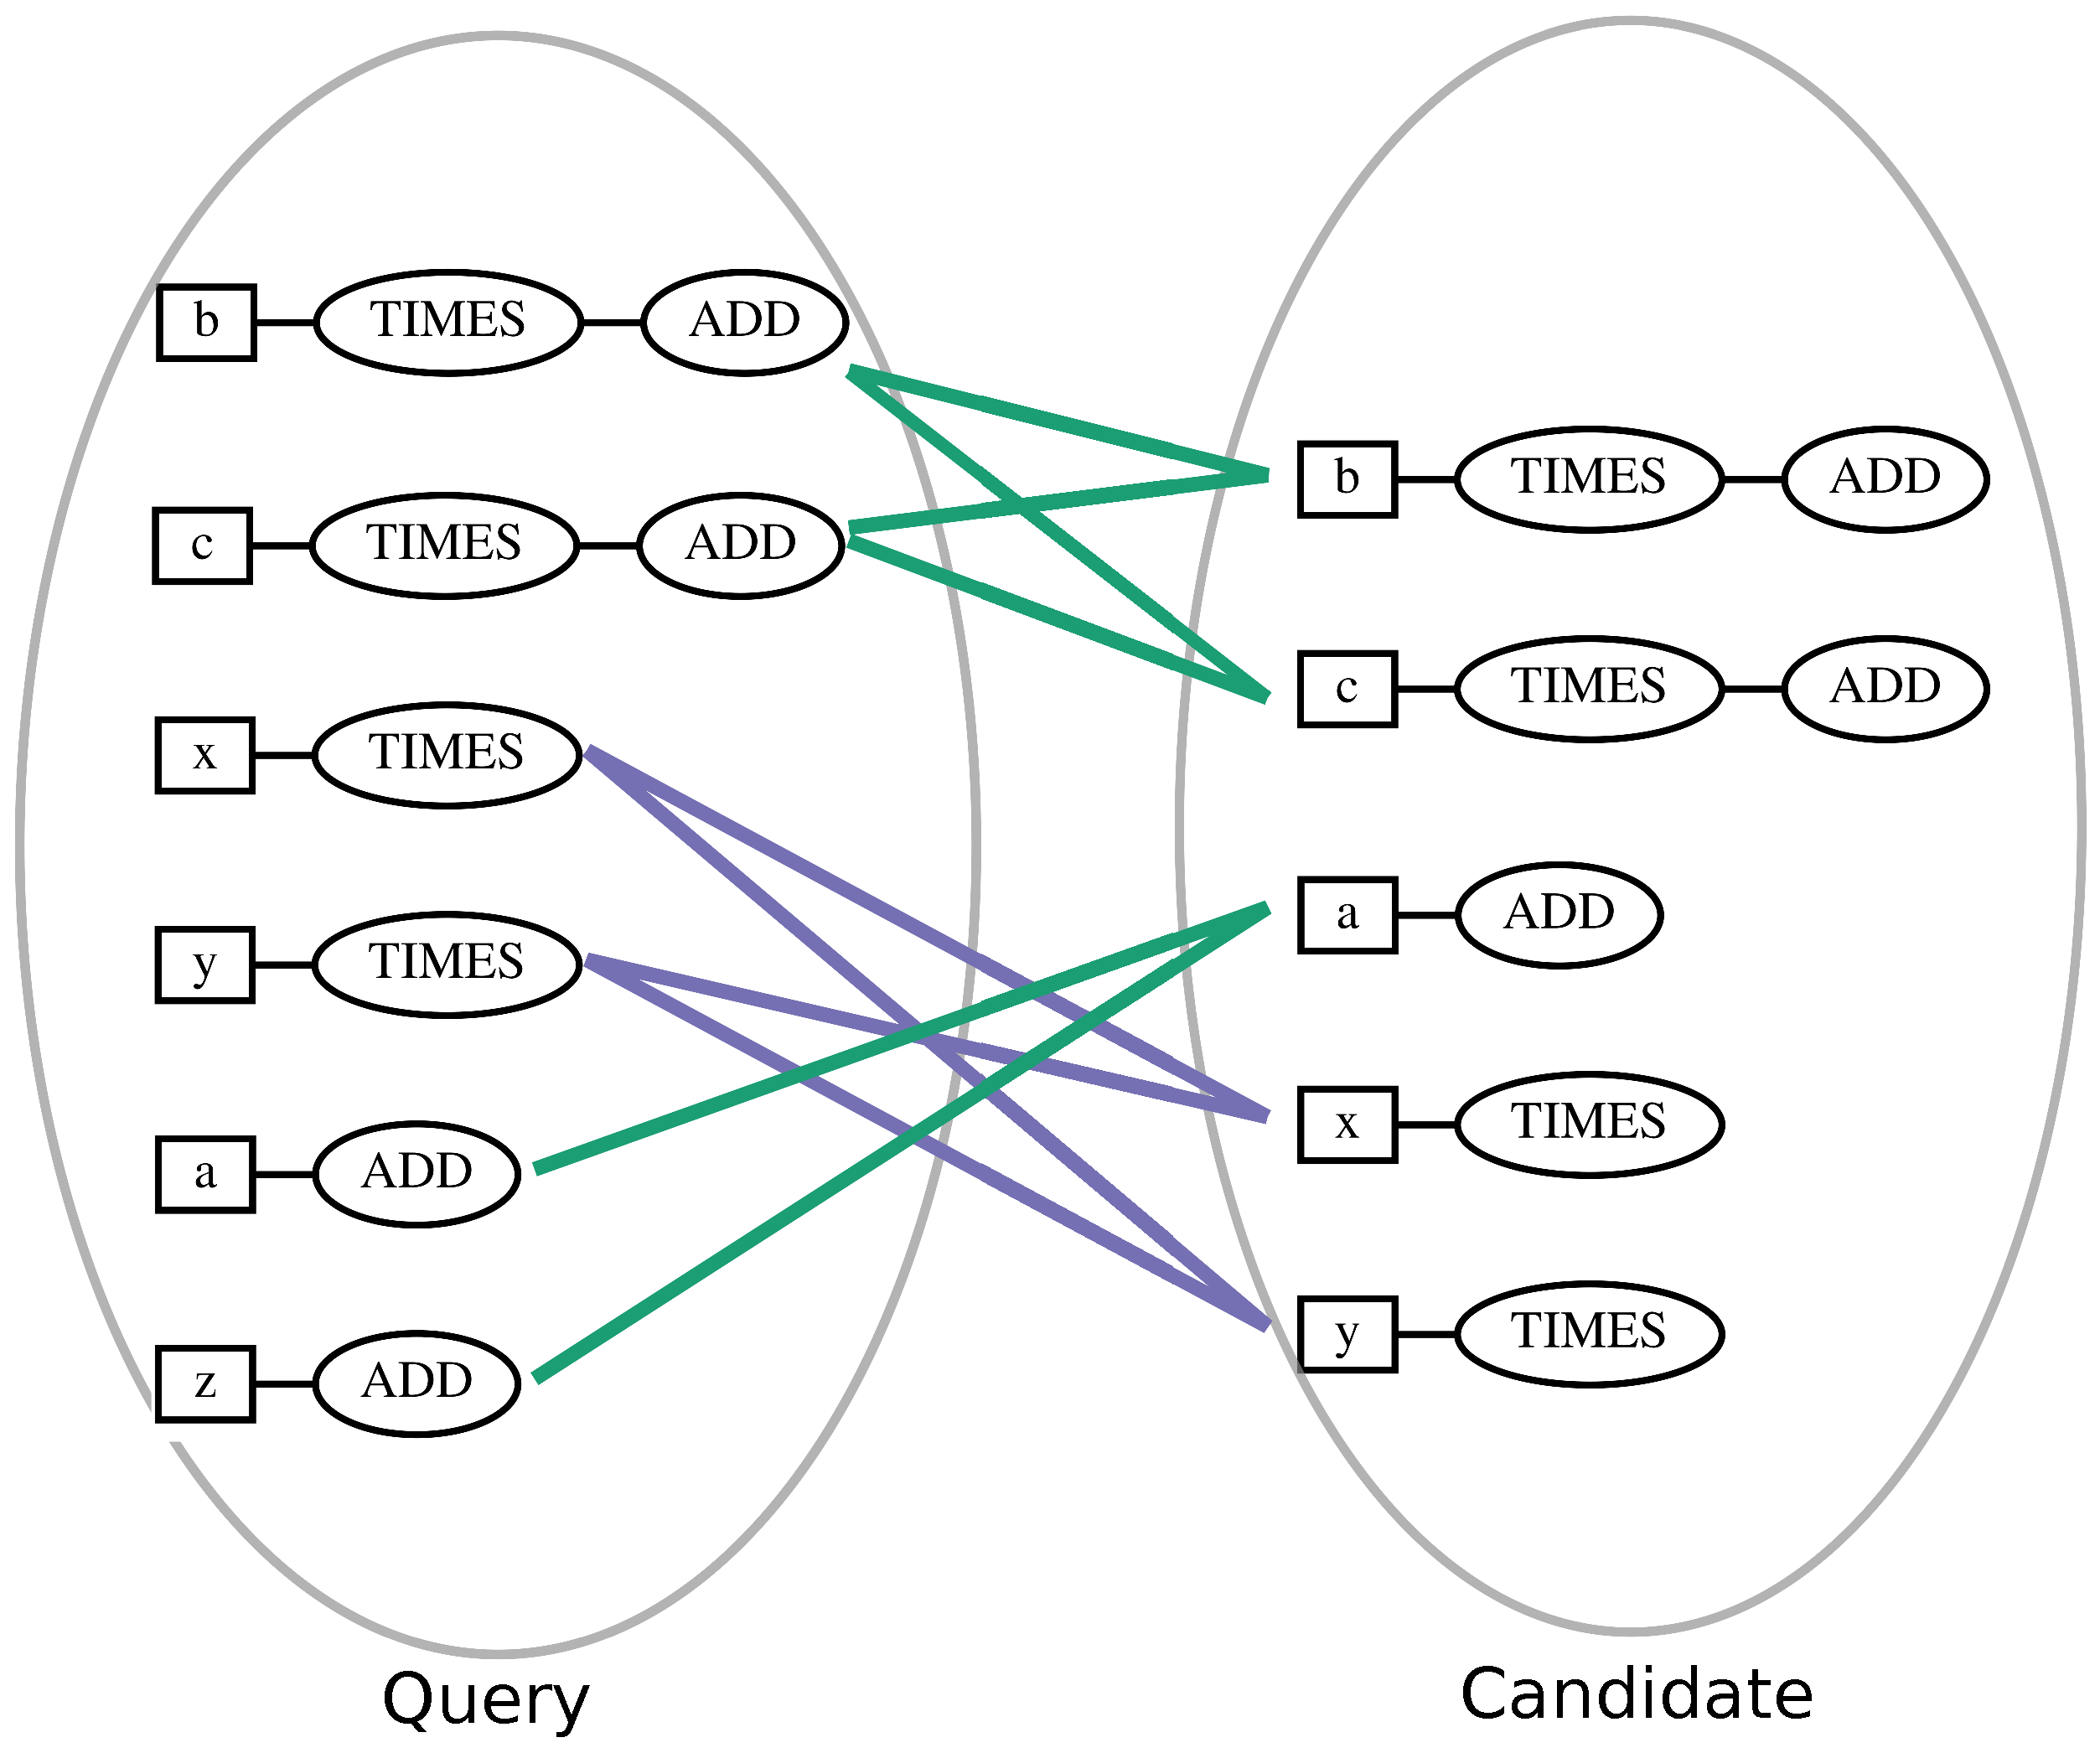
\includegraphics[width=1.84in]{fig/bipartile.eps}
\caption{Bipartite graph of hit path set for formulas in Figure~\ref{intro} (original leaf symbol is used here to help identify paths). Edges are established if paths from the two sides are the same after tokenization. Edges with shared end points (i.e., same root-end nodes) in original OPTs have the same color. }
\label{bipart}
\end{center}
\end{figure}
%%%%%%%%%%%%%%%%%%%%%%%%%%%%%%%%%%%%%%%%%%%%%%%%%%%%%%%%%%%%%%

On the merge of posting lists, a set of corresponding query paths will match a set of paths from a document expression one at a time, each time a \textit{hit path set} consisting of query paths and paths from a document are examined.
%
Define $\mathcal{P}(T)$ to be all the prefix paths we extract from OPT, i.e.,
$\mathcal{P}(T) = \{p: p \in \operatorname{leafroot\_paths}(T^n), n \in T\}$ where $T^n$ is the entire subtree of $T$ rooted at $n$ with all its descendants.
%
We model the hit path set by a bipartite graph 
$G(Q, D, E)$ where $Q = \{q: q \in \mathcal{P}(T_q)\}, D = \{d: d \in \mathcal{P}(T_d)\}$ are query and document path sets, and edge set are ordered pairs $E = \{(q, d): \operatorname{tokenized}(q) =  \operatorname{tokenized}(d), q \in Q, d \in D\}$ representing a potential matching between a query path and a document path.
%%
Since an edge is established when paths are of the same tokens, we can partition the graph into disconnected smaller bipartite graphs $G_t = G(Q_t, D_t, E_t)$, each is identified by tokenized query path $t$ and
$$
\begin{aligned}
Q_t &= \{ q: q \in Q, \operatorname{tokenized}(q) = t\} \\
D_t &= \{d: d \in D, \operatorname{tokenized}(d) = t \} \\
E_t &= \{(q, d): (q, d) \in E, \operatorname{tokenized}(q) = \operatorname{tokenized}(d) \}
\end{aligned}
$$
Figure~\ref{bipart} shows the hit path set graph of the example in Figure~\ref{intro}, this example can be partitioned into disconnected smaller bipartite graphs, associated with tokenized path VAR/TIMES/ADD, VAR/TIMES and VAR/ADD.
Each partition is actually a complete bipartite graph (fully connected) because $\forall e \in (Q_t, D_t), e \in E_t$.
And for each complete bipartite graph $G(V_1, V_2, E)$, we can obtain their maximum matching sizes by calculating $\min(|V_1|, |V_2|)$ easily.

On the other hand, to calculate score $w^*_{Q, D}$, we need to find a pair of query and document nodes at which the optima $\hat{T}^*_q, \hat{T}^*_d$ are rooted (see equation~\ref{eq:2}), such that it is the maximum possible common subtree.
So we also define the matching candidate relations filtered by nodes.
Let $G^{(m, n)} = G(Q^{(m)}, D^{(n)}, E^{(m, n)})$ be subgraph which only considers matching between query node $n$ and document node $m$  where
$$
\begin{aligned}
Q^{(m)} &= \{ q: q \in Q, \operatorname{root\_end}(q) = m\} \\
D^{(n)} &= \{d: d \in D, \operatorname{root\_end}(d) = n\} \\
E^{(m, n)} &= \{(q, d): (q, d) \in E, \operatorname{root\_end}(q) = m, \operatorname{root\_end}(d) = n\} 
\end{aligned}
$$

Because we only need to know the maximum matched subtree width, we can calculate the score of each pair of nodes independently by summing its maximum matching size among partitions and the maximum pair of nodes matching is essentially our interested similarity score $w^*_{Q, D}$.
Specifically,
%
define \textit{token paths} of node $n$ in its tree $T$ as set $\mathfrak{T}(n) = \{t: t = \operatorname{tokenized}(p), p \in \operatorname{leafroot\_paths}(T^n) \}$, it follows
\begin{align}
w^*_{Q, D} &= \max_{m \in T_q, n \in T_d} \; \nu(G^{(m, n)}) \\
           &= \max_{m \in T_q, n \in T_d} \sum_{t \in \mathfrak{T}(m)} \nu(G^{(m, n)}_t) \\
		   \label{eq:5}
           &= \max_{m \in T_q, n \in T_d} \sum_{t \in \mathfrak{T}(m)} \min(|Q^{(m)}_t|, |D^{(n)}_t|)
\end{align}
where $\nu(G)$ is the maximum matching size of bipartite graph $G$.

% And in MaxScore pruning~\cite{jonassen_simon_2011}, the upperbound can be calculated by summing already evaluated partial scores and the (precomputed) accumulated TF-IDF upperbound scores for the rest of the terms.
%
%In our case, $\min(|Q^{(m)}_t|, |D^{(n)}_t|)$ can be defined as partial score, however, our stated structure similarity needs to sum and obtain ``node scores'' and only select the maximum of them.
%%
Denote $w_{m, t} = |Q^{(m)}_t|$, we call $w_{m, t} \ge \min(|Q^{(m)}_t|, |D^{(n)}_t|)$ as a (precomputed) partial score upperbound in our model.
It is analogous to text search where each posting list has a partial score upperbound, the TF-IDF score upperbound is merely sum of them, while in our case we have to sum and only select the maximum of them (we will show this is a great advantage since we can drop posting lists at merge time to reduce our typically large number of posting lists).

In the following we propose three strategies to compute overall similarity upperbound from partial score upperbounds and assign non-requirement set.

\vspace{0.1in}
\noindent \textbf{Max reference (MaxRef) strategy}\;
In MaxScore~\cite{turtle_flood_1995, strohman_turtle_2005}, each posting list can be mapped to a partial score upperbound directly, however, our scoring function implies each posting list can be involved with multiple partial score upperbounds.
One simple way to select the non-requirement set in our case is to provide an upperbound score \emph{MaxRef} (for each posting list $t$) which is the maximum partial score from the query nodes by which this posting list gets ``referenced'', and if a set of posting lists alone has a sum of MaxRef scores less or equal to $\theta$, they can be safely put into the non-requirement set.

The rank safety can be justified, since each posting list corresponds to a unique tokenized path $t$, define $\text{MaxRef}_t = \max_m w_{m, t}$,
$\forall\; m \in T_q, n \in T_d$,
\begin{align}
\label{eq:6}
\sum_t \min(|Q^{(m)}_t|, |D^{(n)}_t|) \le \sum_t w_{m,t} \le \sum_t \text{MaxRef}_t
\end{align}
then the selection of non-requirement set (named \textbf{Skip} set for short) such that 
$\sum_{t \in \textbf{Skip}} \text{MaxRef}_t \le \theta$
follows $w^*_{Q, D} \le \theta$ for all non-requirement set posting lists.

\vspace{0.1in}
\noindent \textbf{Greedy binary programming (GBP) strategies}\;
% \begin{algorithm}[!t]
% \small
% \begin{flushleft}
% \textbf{Input}: $\mathbf W, \mathbf L, \theta$ where $\mathbf L$ is objective function coefficients \\
% \textbf{Output}: $I, p$ indicating the assignment of posting lists \\
% I[1 : p] are posting lists IDs in requirement set; \\
% I[(p + 1) : n] are posting list IDs in \textbf{Skip}.
% \end{flushleft}
% \caption{Greedy solver for problem in GBP}
% \label{alg0}
% \begin{algorithmic}[1]
% 
% \Function{SolveRecur}{$\mathbf W, \mathbf L, \theta$, I, p}
% \State n := len($\mathbf L$)
% \If {p $\ge$ n}
% 	\State \Return I, p
% 	\Comment{All in requirement set.}
% \EndIf
% \State $\boldsymbol x$ := $\{x_i\}_{n \times 1}$ where [1 : p] are zeros, [p + 1: n] are ones.
% \State r := row in $\mathbf W \boldsymbol x$ that violates the constraints the most.
% \If {no row violates constraints}
% 	\State \Return I, p
% 	\Comment{This is a feasible solution.}
% \EndIf
% 
% \State c := a column such that $(\mathbf L \circ \boldsymbol x^T)_c$ is minimal and $\mathbf W_{r, c} > 0$
% \State swap column c and p in $\mathbf W, \mathbf L$ and $I$
% \Comment{Take out $c$ heuristically.}
% \State p := p + 1
% \State \Return \Call{SolveRecur}{$\mathbf W, \mathbf L, x, \theta$, p}
% \EndFunction
% 
% \Function{Solve}{$\mathbf W, \mathbf L, \theta$}
% \State p := 0
% \Comment{An index pivot of requirement vs. non-requirement set.}
% \State I := index vector [1 : len($\mathbf L$)]
% \Comment{Length of $\mathbf L$ is essentially $|\mathfrak{T}|$.}
% \For {each column j in $\mathbf W$} 
%     \Comment{Take out those obviously not in \textbf{Skip}.}
% 	\State m := maximum element of column j in $\mathbf W$
% 	\If {m $> \theta$}
% 	\State swap column j and p in $\mathbf W, \mathbf L$ and $I$
% 	\State p := p + 1
% 	\EndIf
% \EndFor 
% \State \Return \Call{SolveRecur}{$\mathbf W, \mathbf L, \theta$, I, p}
% \EndFunction
% \end{algorithmic}
% \end{algorithm}
%
Inequality~(\ref{eq:6}) is relaxed twice, so it spurs the motivation to get tighter upperbound value by maximizing posting lists in non-requirement set (so that more posting lists are likely to be advanced directly).
Define partial upperbound matrix $\mathbf{W} = \{ w_{i, j} \}_{|T_q| \times |\mathfrak{T}|} $ where $\mathfrak{T} = \{ \mathfrak{T}(m), m \in T_q \}$ are all the token paths from query OPT ($\mathfrak{T}$ is essentially the same as tokenized $\mathcal{P}(T_q)$), and a binary variable $\boldsymbol{x}_{|\mathfrak{T}| \times 1}$ indicating which corresponding posting lists are taken into non-requirement set.
One heuristic objective is to maximize the number of posting lists in non-requirement set (we call this strategy GBP-NUM):
\begin{align}
\label{eq:obj}
\text{maximize} && \mathbf{1} \cdot \boldsymbol{x} \\
\label{eq:7}
s.t.            && \mathbf{W} \boldsymbol{x} \le \theta
\end{align}

However, getting maximum number of posting lists into non-requirement set does not necessarily cause more items being skipped because those posting lists can be very short.
As a result, we can maximize the total length of posting lists in non-requirement set instead, in this case the all-one vector in objective function~(\ref{eq:obj}) is replaced with posting list length vector
$\mathbf{L} = \begin{bmatrix} L_1, L_2, \ldots L_{|\mathfrak{T}|}\end{bmatrix}$ where $L_i$ is the length of posting list $i$.
We call this strategy GBP-LEN.
%
The two GBP strategies are rank-safe % because $\forall\; m \in T_q, n \in T_d$,
% \begin{align}
% \label{eq:9}
% \sum_t \min(|Q^{(m)}_t|, |D^{(n)}_t|) \le \sum_t w_{m,t}
% \end{align}
since constraints in inequalities~(\ref{eq:7}) demands $\sum_{t \in \textbf{Skip}} w_{m,t} \le \theta$.

Both binary programming strategies require solving binary programming problem which is known to be NP-complete thus too heavy to run for long queries.
Therefore at implementation we just greedily follow one branch of the binary programming sub-problems to get a greedy solution running in $O(|T_q| |\mathfrak{T}|^2)$.
Greedy solutions also meet these constraints, thus it is still rank-safe.
%the local optimal may not maximize objective function~(\ref{eq:obj}) but still satisfy constraints~(\ref{eq:7}).

% \subsection{Initial threshold}
% In addition to pruning strategies above, we define an \textit{initial threshold} (static value), requiring a minimal score for any hit to make it into the top K.
% We multiply the query formula size by a \textit{threshold factor} ($\in [0, 0.5]$) as initial threshold $\theta_0$.
% If initial threshold is set to zero, it is rank-safe pruning, otherwise it further boosts efficiency by allowing more pruning possibilities.
% %
% The motivation for this strategy, especially in structural search, is the size difference between query and document OPTs makes a significant impact to similarity,
% unlike TF-IDF scoring where the impact of matched terms depends on both frequency and rareness, a long query can still be relevant to document with single term as long as that term is rare, however, in our case the similarity score is measured by common structure size, it is much unlikely that a large OPT query will make a small matched document OPT into top K results.







%%%%%%%%%%%%%%%%%%%%%%%%%%%%%%%%%%%%%%%%%%%%%%%%%%%%%%%%%%%
\section{Implementation}
%\subsection{Indices structure}

Figure ~\ref{figillu} illustrates our query processing and modified inverted index for dynamic pruning of formula search.
For each internal node $m$ of the query OPT, we store the number of leaves of $m$  as $w_m = |Q^{(m)}|$, the two numbers are denoted by $m/w_m$.
Each query node refers to one or more tokenized path entries in a dictionary,
where each reference is associated with $Q^{(m)}_t$ identified by query $m$ and tokenized path $t$.
%
In Figure~\ref{figillu}, node $q1$ from the query has 6 leaves, which is also the upperbound number of path matches for $q1$, i.e, $|Q^{(1)}|$.
Since $q1$ consists of 2 tokenized leaf-root paths VAR/TIMES/ADD and VAR/ADD,
$q1$ is linked to two posting lists, each associated with a partial upperbound $w_{m, t} = |Q^{(m)}_t|$.

Each posting list corresponds to a token path $t \in \mathfrak{T}$ and has one dynamic reference counter indicating the number of query nodes referring to it (initially $|Q_t|$).
As query nodes can be pruned by our algorithm (when its width is no longer greater than the current threshold, the corresponding subexpression cannot make it into top-K results),
the reference counter may decrease, and the posting list gets removed if its reference counter is less than one.
%The greatest $w$ value of all LSSs by which a posting list (or path entry) gets referenced is the \emph{MaxRef} (however, \emph{MaxRef} is not used when we use GBP strategies).
%In our implementation, we do not directly manipulate posting lists, instead, they are represented by \textit{iterators}  which store independent copies of current merging state (e.g., current ExpID) to allow reentrant reading.
For ease of testing termination, we append a very large ExpID \emph{MaxID} at the end, this special ID is greater than any ExpID of real document expression.
%
Each posting list entry identified by an ExpID stores $n, |D^{(n)}_t|$ values extracted from document subtree token path $t$ rooted at $n$.

As an example, in Figure~\ref{figillu}, the hit OPT shown at right (of ExpID 12) has 5 paths tokenized as VAR/TIMES/ADD, 2 on the left rooted by $d4$ and 3 on the right rooted by $d1$. The information ($d1/3, d4/2$) are stored with the corresponding posing list.
In our implementation, each posting list is traversed by an iterator ($iters[t]$), and its entry information (denoted as $n/w_n$) are read by $iters[t].read()$ function from current position accessed by iterator.

%%%%%%%%%%%%%%%%%%%%%%%%%%%%%%%%%%%%%%%%%%%%%%%%%%%%%%%%%%%%%%%%
\begin{figure*}[!t]
\begin{center}
\hspace*{-0.6in}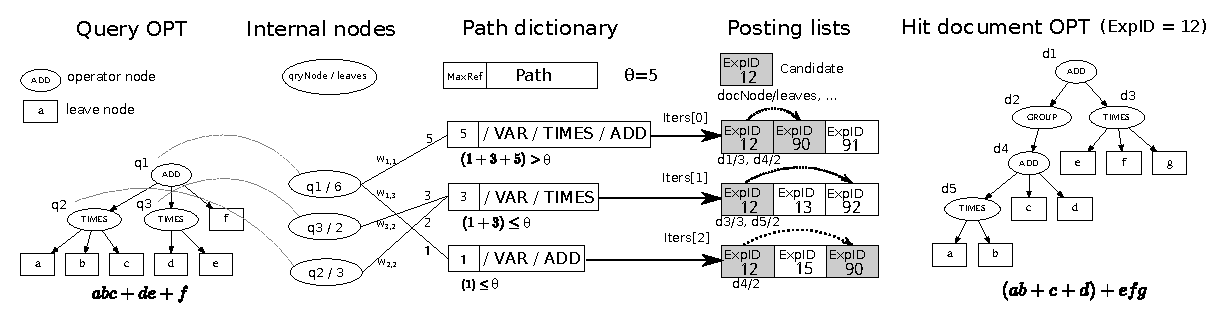
\includegraphics[height=1.5in]{fig/drawing.eps}
\caption{Indices for formula search with dynamic pruning. The top posting list is the only one in requirement set using strategy MaxRef, and the bottom two are advanced by skipping to candidate ExpID.}
\label{figillu}
\end{center}
\end{figure*}
%%%%%%%%%%%%%%%%%%%%%%%%%%%%%%%%%%%%%%%%%%%%%%%%%%%%%%%%%%%%%%%%

%%%%%%%%%%%%%%%%%%%%%%%%%%%%%%%%%%%%%%%%%%%%%%%%%%%%%%%%%%%%%%%%
\begin{algorithm}[!b]
\scriptsize
\caption{Formula tree searching algorithm with pruning}
\label{alg1}
\begin{algorithmic}[1]
\Function{qryNodeMatch}{iters, $m$, candidate, widest, $\theta$}
	\State nodeMatch[ ] := $\vec{0}$; $\ell$ := $|\operatorname{leaves}(m)|$
	\Comment{$\ell$ is the leftover estimated upperbound.}
 	\For {each $m/w_m$ of tokenized path $t$ rooted at $m$}
 	    \State Let $i$ be the iterator index associated with $t$
		\If {iters[$i$].docID $<$ candidate}
			\State iters[$i$].skipTo(candidate)
		\EndIf
		\If {iters[$i$].docID $=$ candidate }
		\For {each $n/w_n \;\text{of}\; t$ from iters[$i$].read() }
 			\State nodeMatch[$n$] := nodeMatch[$n$] + min($w_m$, $w_n$)
 		\EndFor
		\EndIf
		\State $\ell$ := $\ell - w_m$; estimate := max(nodeMatch) + $\ell$ 
		\Comment{Update estimation.}
		\If {estimate $\le$ widest \textbf{or} $u$(estimate) $\le \theta$}
			\State \Return 0
		\EndIf
 	\EndFor
 	\State \Return max(nodeMatch)
\EndFunction
~\\
\Function{FormulaSearch}{iters, strategy}
	\State $\theta$ := $0$; reqs := \Call{RequirementSet}{$\theta$, strategy}
	\State heap := data structure to hold top K results
	\While {true}
		\State candidate := minimal ID in current expIDs of reqs
		\If {candidate equals MaxID}
            \Comment{Search terminated, return results.}
			\State \Return top K results
		\EndIf
		\State Let $G(Q, D, E)$ be the path set bipartite graph.
		\State widest := 0; hitNodes := $\{\operatorname{root\_end}(q): (q, d) \in E \}$
		\For {$m$ in hitNodes}
            \Comment{Calculate maximum match for each hit query node.}
			\If {$|\operatorname{leaves}(m)|$ $\le$ widest}
				\State \textbf{continue}
			\EndIf
			\State maxMatch := \Call{qryNodeMatch}{iters, $m$, candidate, widest, $\theta$}
			\If {maxMatch $>$ widest} widest := maxMatch \Comment{Find the widest width.} \EndIf
		\EndFor
		\If {widest $> 0$}
		    \State score := calculate final score (including symbol similarity).
			\Comment{See [23].}
			\If {heap is not full {\bf or} score $> \theta$}
				\State Push candidate or replace the lowest scored hit in heap.
				\If {heap is full}
				\Comment{Update current threshold.}
					\State $\theta$ := minimal score in current top K results
					\State Drop small query nodes and unreferenced iterators.
					\State reqs := \Call{RequirementSet}{$\theta$, strategy}
					\Comment{Update requirement set.}
				\EndIf
			\EndIf
		\EndIf

		\For {iters[$i$] in reqs}
            \Comment{Advance posting list iterators.}
			\If {iters[$i$].docID = candidate}
				iters[$i$].next()
			\EndIf
		\EndFor
	\EndWhile
\EndFunction
\end{algorithmic}
\end{algorithm}
%%%%%%%%%%%%%%%%%%%%%%%%%%%%%%%%%%%%%%%%%%%%%%%%%%%%%%%%%%%%%%%%

Query processing is described in Algorithm~\ref{alg1}.
The \Call{RequirementSet}{} returns selected iterators of the requirement set (complement of the non-requirement set).
The assignment according to different pruning strategies is described in Section~\ref{strategy}.
%
In MaxRef strategy, we sort posting lists in descending order of their $\text{MaxRef}$ values, and take as many posting lists into non-requirement set from lowest $\text{MaxRef}$ value.
At merging, a \textit{candidate} is selected from the hit posting lists of the requirement set which have the minimal ExpID.
Requirement set iterators are advanced one by one using \textit{next()} function, while iterators in the non-requirement set are advancing directly to the ID equal to or greater than the current candidate using \textit{skipTo()} function. In Figure~\ref{figillu} for example, the posting list corresponding to VAR/TIMES/ADD is in the requirement set under the MaxRef strategy, while the other two are not: Document expression 13 and 15 will be skipped if the next candidate is 90.

At each iteration, a set of \textit{hitNodes} is inferred containing query nodes associated with hit posting lists (i.e., those current ExpIDs are candidate IDs).
\Call{qryNodeMatch}{} calculates the match of each hit node according to equation~\ref{eq:5}, pruning those nodes whose maximum matching size will be smaller than the matched size of any already calculated node.
%
Given query hit node $q1$ in Figure~\ref{figillu}, function \Call{qryNodeMatch}{} returns value of
$$\max_{n\in T_d}\;\nu(G^{(1, n)}) = \max(\min(5, 2) + \min(1, 2),\; \min(5, 3)) = 3$$
Then the algorithm selects the best matched query node and its matched width (\emph{widest}) is our interested structural similarity $w^*_{Q, D}$.

After obtaining $w^*_{Q, D}$, we additionally calculate an \emph{overall similarity score}~\cite{a0_2019} as the final score for ranking which further considers symbolic similarity (e.g., to differentiate $E=mc^2$ and $y=ax^2$) and also penalizes oversized candidate document.
Because of this additional layer, we need to relax our upperbound further.
According to \cite{a0_2019}, the relaxing function $u$ is defined as
\begin{equation}
u(w) = \frac{w}{|\text{leaves}(T_q)| + w} \left[ (1 - \eta) + \eta \, \frac 1 {\log (1 + n_d)} \right]
\end{equation}
where in our setting,  parameters $\eta = 0.05, n_d = 1$.

Whenever threshold $\theta$ is updated, we will examine all the query nodes, if a query node $m$ has an upperbound less or equal to threshold, i.e., $u(m) \le \theta$, then the corresponding subtree of this node is too ``small'' to make it into top K results, so we will drop these small nodes. As a result, some of the posting lists (or iterators) may also be dropped due to zero reference.

\section{Evaluation}
%%%%%%%%%%%%%%%%%%%%%%%%%%%%%%
\begin{table*}[!b]
\small
	\centering
    \caption{Query merge time performance (in milliseconds) of different strategies.}
	%, returning different maximum number of results (K value), on two dataset Wikipedia (Wiki) and Math StackExchange (MSE).}
	\resizebox{\textwidth}{33mm}{
	\begin{tabular}{lrl|ccccc|ccccc}
	\toprule
	\multicolumn{3}{c|}{\bf{Runs}} &
	\multicolumn{5}{c|}{\bf Non-wildcards} & \multicolumn{5}{c}{\bf Wildcards} \\
	& \bf K & \bf Strategy &
	\bf $\mu$ & \bf $\sigma$ & \bf median & \bf min & \bf max & 
	\bf $\mu$ & \bf $\sigma$ & \bf median & \bf min & \bf max \\
	\hline
	% wiki&base&100
	% & avg & std & med & min & max & avg & std & med & min & max \\
	%%%%%%%%% INSERT BELOW %%%%%%%%%%
	\multirow{10}{*}{ \rotatebox[origin=c]{90}{Wiki Dataset}   }

& 100 & Baseline
& 540.12& 569.44& 360.50& 7.00& 2238.00& 426.73& 383.47& 225.50& 8.00& 1338.00\\

	\cline{2-13}

& 100 & MaxRef
& 90.29& 74.14& 79.00& 3.00& 312.00& 145.50& 121.19& 136.00&\bf 7.00& 573.00\\
&  & GBP-NUM
& 84.90& 80.44& 52.50& 3.00& 321.00& 138.82& 102.55& 135.00& 9.00& 428.00\\
&  & GBP-LEN
& \bf 67.49& \bf 61.40& \bf 45.00& \bf 2.00& \bf 218.00& \bf 125.27&\bf 97.28&\bf 103.50& 9.00& \bf 404.00\\

	\cline{2-13}

& 200 & MaxRef
& 107.71& \bf 82.64& 102.00&\bf 5.00&\bf 322.00& 160.10& 121.40& 149.00& 9.00& 583.00\\
&  & GBP-NUM
& 105.34& 99.51& 71.50&\bf 5.00& 357.00& 155.52& 110.61& 153.00& \bf 8.00& 479.00\\
&  & GBP-LEN
& \bf 89.63& 83.20& \bf 62.00& \bf 5.00& 330.00& \bf 142.78& \bf 103.11& \bf 143.50& 9.00& \bf 446.00\\

	\cline{2-13}

& 1000 & MaxRef
& 154.51& \bf 93.75& 157.50& \bf 6.00& \bf 361.00& 211.86& 140.01& 186.00& 10.00& 662.00\\ 
&  & GBP-NUM
& 159.80& 143.70& 120.50& \bf 6.00& 626.00& 208.91& 136.42& 178.50& 10.00& 591.00\\ 
&  & GBP-LEN
& \bf 144.25& 126.95& \bf 105.00& \bf 6.00& 622.00& \bf 195.70& \bf 122.25& \bf 176.00& \bf 9.00& \bf 536.00\\ 

	\midrule
	\midrule
	\multirow{10}{*}{ \rotatebox[origin=c]{90}{MSE Dataset}   }

& 100 & Baseline
& 15134.10& 15186.78& 11161.00& 157.00& 55499.00& 13450.57& 12554.19& 7075.50& 304.00& 47513.00\\

	\cline{2-13}

& 100 & MaxRef
& 1083.23& 1274.23& 745.50& 28.00& 5922.00& 3188.66& 2458.91& 2925.00& 85.00& 10412.00\\
&  & GBP-NUM
& 1202.24& 1240.21& 815.00& 37.00& 4987.00& 2943.79& 2025.96& 2987.00&\bf 84.00& 8775.00\\
&  & GBP-LEN
& \bf 562.83& \bf 635.26& \bf 382.50&\bf 24.00&\bf 2313.00&\bf 2257.95&\bf 1491.59&\bf 2346.50& 86.00& \bf 4494.00\\


	\cline{2-13}

& 200 & MaxRef
& 1261.21& 1368.93& 1012.50& 30.00& 6439.00& 3416.77& 2753.09& 3032.50& 160.00& 12412.00\\
&  & GBP-NUM
& 1378.19& 1398.08& 998.50& 39.00& 5863.00& 3174.93& 2283.05& 3125.00& \bf 159.00& 10099.00\\
&  & GBP-LEN
& \bf 697.32&\bf 739.11& \bf 478.00& \bf 27.00& \bf 2925.00& \bf 2504.90& \bf 1683.16& \bf 2382.50& \bf 159.00& \bf 6049.00\\

	\cline{2-13}

& 1000 & MaxRef
& 2030.05& 1746.17& 1796.50& 53.00& 7816.00& 4123.26& 3510.01& 3473.00& 287.00& 16981.00\\ 
&  & GBP-NUM
& 1952.52& 1746.05& 1530.50& 60.00& 7197.00& 3786.89& 2744.99& 3493.50& \bf 281.00& 11323.00\\ 
&  & GBP-LEN
& \bf 1217.16& \bf 1083.53&\bf 764.50&\bf 47.00&\bf 3756.00&\bf 3304.69&\bf 2403.09&\bf 2812.00& 285.00& \bf 9895.00\\ 

	%%%%%%%%% INSERT ABOVE %%%%%%%%%%
	\bottomrule

	\end{tabular}
	}
\label{majortab}
\end{table*}
%%%%%%%%%%%%%%%%%%%%%%%%%%%%%%
We first evaluate our system~\footnote{Source code: \url{https://github.com/approach0/search-engine/tree/ecir2020}} on the NTCIR-12 Wikipedia Formula Browsing Task~\cite{ntcir12} (NTCIR-12 for short), which is the most current benchmark for formula-only retrieval.
The dataset contains over 590,000 math expressions taken from English Wikipedia.
%
Since work in formula retrieval is relatively new, there are only 40 queries in NTCIR-12 that can be compared with other published systems. However, these queries are well designed to cover a variety of math expressions in different complexity and it is still meaningful to compare for efficiency evaluation. There are 20 queries containing wildcards (using wildcard specifier \textbf{\textbackslash{}qvar} to match arbitrary subexpression or symbols, e.g., query ``\textbackslash qvar\{a\} + \textbackslash qvar\{b\}'' can match ``$x^2 + (y + 1)^3$'').

We add support for wildcards by simply treating internal nodes (representing a rooted subexpression) of indexing formula as additional ``leaves'' (by ignoring their descendants), and the wildcard specifiers in a query are treated as normal leaves to match those indexed wildcard paths.
Since the corpus of NTCIR-12 is not large enough to show the full impact of pruning, we also evaluate query run times on a corpus containing over 1 million math related documents/threads from Math StackExchange (MSE) Q\&A website\footnote{Dataset: \url{https://approach0.xyz/ecir2020/mse-corpus.tar.gz}} and we run the same query set from NTCIR-12.
%
Run times are measured only for posting lists merging stage (e.g., time cost for parsing query into OPT are excluded) and unless specified, evaluating posting lists are compressed and cached into memory.
%
Experiment consists of five independent runs for each system and we take the results from overall distribution.

Table~\ref{majortab} reports run time statistics of different strategies.
Non-pruning (exhaustive search) baselines with K = 100 are also compared here.
Almost consistently, GBP-LEN strategy achieves the best efficiency with smaller variance.
This is expected since GBP-LEN objective function models the skipping possibility better than GBP-NUM, although GBP-NUM gives a tighter theoretic upperbound than MaxRef, it only maximizes the number (instead of the size) of posting lists in the non-requirement set, and may lead to bad performance when these posting lists are short.

There are a few times the best minimal run times are led by other strategies, for those with meaningful gaps, i.e., in Wiki dataset of non-wildcard queries when K = 1000, MaxRef outperforms in standard deviation and maximum run time to a notable margin; however, it is likely results from small threshold due to large K so that the efficiency on a small sized NTCIR dataset is less affected by pruning (small $\theta$ means less pruning potential) compared to the time complexity added from assigning requirement set, the latter is more significant in GBP runs. In wildcard queries, however, many expressions can match the query thus threshold value is expected to be larger than that in non-wildcard case.
%%%%%%%%%%%%%%%%%%%%%%%%%%%%%%
\begin{figure*}[!t]
\begin{center}

\hspace*{-3.6cm} \resizebox{\textwidth}{!}{

	\begin{minipage}[b]{1.5in}
	\resizebox{\textwidth}{0.29in}{
	\begin{tabular}{l|cc|cc|cc}
	\toprule
	\multirow{2}{*}{\bf{System}}
	& \multicolumn{2}{c|}{\bf Non-Wildcard}
	& \multicolumn{2}{c|}{\bf Wildcard}
	& \multicolumn{2}{c}{\bf All queries} \\
	& Full& Partial
	& Full& Partial
	& Full& Partial \\
 	\toprule
 	MCAT                &     .5678 &     .5698 & \bf .4725 &     .5015 &     .5202 &     .5356 \\
{Tangent-S} &     .6361 &     .5872 &     .4699 & \bf .5368 & \bf .5530 & \bf .5620 \\
{base-best} & \bf .6726 & \bf .5950 &     -     &      -    &      -    &       -   \\
{base-opd-only} & .6586 &   .5153 &     -     &      -    &      -    &       -   \\
 	Ours (pruning)&     .6586 &     .5173 &     .3678 &     .3973 &     .5132 &     .4573 \\
 	Ours (exhaustive)&     .6586 &     .5173 &     .3678 &     .3973 &     .5132 &     .4573 \\
 	\bottomrule
	\end{tabular}
	}
	\end{minipage}

\hspace*{-0.1in}

	\begin{minipage}[b]{1.1in}
	\includegraphics[height=0.6in]{fig/boxplot.eps}
	\vspace{-0.43in}
	\end{minipage}
}

\caption{Bpref~\cite{buckley2004retrieval} scores (on the left) and average run times (on the right) compared with other formula search systems on NTCIR-12 Wiki dataset where K = 1000.
(Bpref measure is chosen here because we did not participate in NTCIR-12 and contribute to the pooling, and Bpref scores only considers judged documents).
}
\label{boxplot}
\end{center}

\end{figure*}
%%%%%%%%%%%%%%%%%%%%%%%%%%%%%%%%%%%%%%%%%%%%%%%%%%%%%%%%%%%%%%%

Secondly, we have compared our system effectiveness and efficiency with Tangent-S~\cite{tangent-combine2017}, MCAT~\cite{mcat_16} and our baseline system without pruning~\cite{a0_2019} systems (see Figure~\ref{boxplot}), all of which are also structure-based formula search engines and they have obtained the best published Bpref scores on NTCIR-12 dataset.
In addition, ICST system~\cite{peking2016} also obtains effective results for math and text mixed task, but they do training on previous Wiki dataset and their system is currently not available.

All compared systems are evaluated on the same host in a single thread for top-1000 results.
% The computational environment is: Intel Core i5 @ 3.60GHz per core, 16 GB memory and SSD hard drive.
%
We use our best performance strategy, i.e., GBP-LEN, having an on-disk version with posting lists uncompressed and always read from disk, and an in-memory version with compression.
%
For baseline system, only 20 non-wildcard queries are reported because it does not support wildcard query.
We compare baseline best performed run (base-best) which uses costly multiple tree matching and its specialized version (base-opd-only) which is comparable to our system because its scoring only considers single best matched tree width (see equation~\ref{eq:2}).
%
Tangent-S has a few significant outliers as a result of its costly alignment algorithm to rerank structure and find the Maximum Subtree Similarity~\cite{tangent-multistage2016}, its non-linear complexity makes it expensive for some long queries (especially in wildcard case).
%
And MCAT reportedly has a median query execution time around 25 seconds, using a server machine and multi-threading~\cite{mcat_16}.
So we remove Tangent-S significant outliers and MCAT from runtime boxplot.
To save space, we only include the faster run base-opd-only from baseline.

As our results suggest, we outperform Tangent-S in efficiency even if we exclude their outlier queries, with higher Bpref in non-wildcards fully relevant results. Our efficiency is also better than baseline even if it only considers less complex non-wildcard queries.
%
However, our overall effectiveness is skewed by bad performance of wildcard queries because a much more expensive phase is introduced to boost accuracy by other systems to handle inherently difficult ``structrual wildcards''.
We think it is still an open problem to handle structure wildcard queries effectively in real time.

Our pruning strategies are rank-safe (pruning and exhaustive version shows the same Bpref scores) but there is a minor Bpref difference between ours and baseline (base-opd-only) due to parser changes we have applied to support wildcards (e.g., handle single left brace array as seen in a wildcard query) and they happen to slightly improve accuracy in partially relevant cases.


%%%%%%%%%%%%%%%%%%%%%%%%%%%%%%%%%%%%%%%%%%%%%%%%%%%%%%%%%%%%%%%
% \begin{figure}[]
% \begin{center}
% 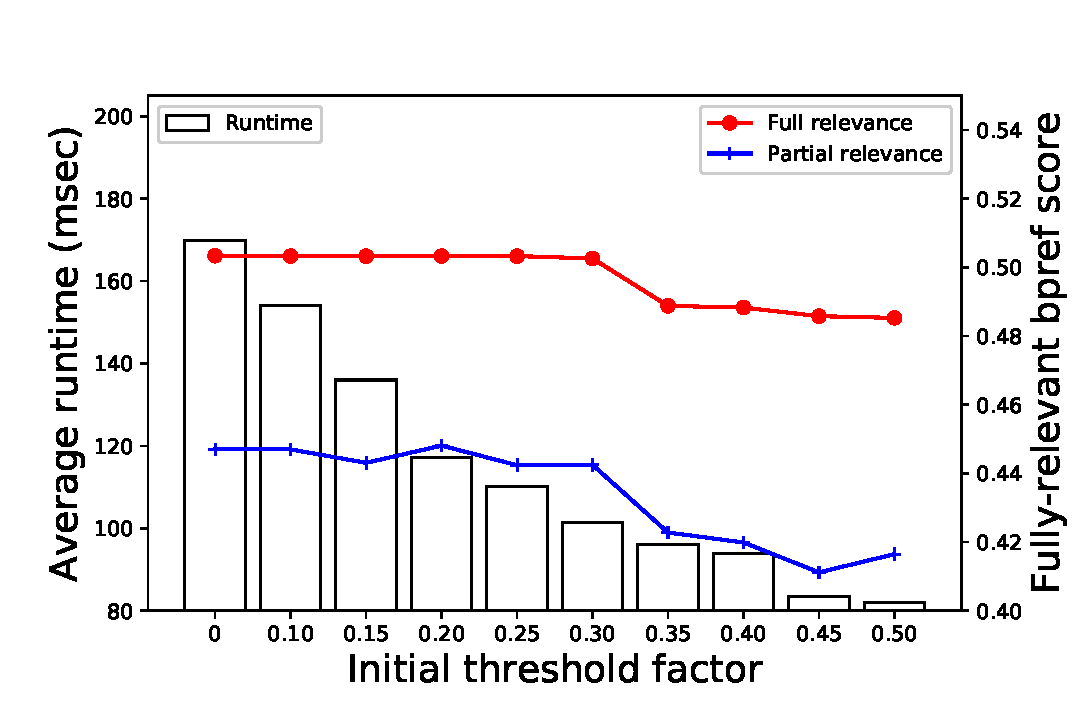
\includegraphics[height=1.6in]{fig/theta-factors.eps}
% \caption{Effect of initial thresholds on performance. The left axis shows run times in msecs (bars), the right axis shows Bpref scores (lines).}
% \label{thresholds}
% \end{center}
% \end{figure}
%%%%%%%%%%%%%%%%%%%%%%%%%%%%%%%%%%%%%%%%%%%%%%%%%%%%%%%%%%%%%%%%

% Lastly, we have evaluated the impact of initial thresholds, we use GBP-LEN to examine query run times and effectiveness in Bprefs affected by increasing initial threshold factor.
% %
% Results shown in Figure \ref{thresholds} verifies our assumption that small initial threshold factor is unlikely to affect effectiveness in structure similarity search.
% Although partial relevance scores are a little undulate, it only decreases notably after the initial threshold factor goes beyond 0.3.
% Full relevance line has the same pivot before starting to plunge, however, it stays almost unaffected by initial thresholds until the pivot.
% Although being simple, initial threshold can be used to achieve faster query time with low risk of sacrificed high structural relevance.

\section{Conclusion}
We have presented rank-safe dynamic pruning strategies that produce an upperbound estimation of structural similarity in order to speedup formula search using subtree matching.
Our dynamic pruning strategies and specialized inverted index are different from traditional linear text search pruning methods and they further associates query structural representation with posting lists.
% We evaluate our query merge times of different strategies, and compare ours with the most effective systems on the NTCIR-12 Wikipedia Formula Browsing Task.
Our results show we can obtain substantial improvement in efficiency over the baseline model, while still generating highly relevant non-wildcard search results.
Using our approach, we can process a diverse set of structural queries in real time.
% ---- Bibliography ----
\bibliographystyle{splncs04}
\bibliography{rpa}
\end{document}
